\documentclass[a4paper]{article}

% --- Packages ---

\usepackage{a4wide}
\usepackage[utf8]{inputenc}
\usepackage{amsmath}
\usepackage{mathtools}
\usepackage{amssymb}
\usepackage[english]{babel}
\usepackage{mdframed}
\usepackage{systeme,}
\usepackage{lipsum}
\usepackage{relsize}
\usepackage{caption}
\usepackage{tikz}
\usepackage{tikz-3dplot}
\usetikzlibrary{shapes.geometric}
\usepackage{pgfplots}
\usepackage{pgfplotstable}
\pgfplotsset{compat=newest}%1.7}
\usepackage{harpoon}%
\usepackage{graphicx}
\usepackage{wrapfig}
\usepackage{subcaption}
\usepackage{authblk}
\usepackage{float}
\usepackage{listings}
\usepackage{xcolor}
\usepackage{chngcntr}
\usepackage{amsthm}
\usepackage{comment}
\usepackage{commath}
\usepackage{hyperref}%Might remove, adds link to each reference
\usepackage{url}
\usepackage{calligra}

% --- Bibtex ---

%\usepackage[backend = biblar,]{bibtex}

%\addbibliografy(ref.bib)

% --- Commands --- 

\newcommand{\w}{\omega}
\newcommand{\trace}{\text{Tr}}
\newcommand{\grad}{\mathbf{\nabla}}
%\newcommand{\crr}{\mathfrak{r}}
\newcommand{\laplace}{\nabla^2}
\newcommand{\newparagraph}{\vspace{.5cm}\noindent}

% --- Math character commands ---

\newcommand{\curl}[1]{\mathbf{\nabla}\times \mathbf{#1}}
\newcommand{\dive}[1]{\mathbf{\nabla}\cdot \mathbf{#1}}
\newcommand{\res}[2]{\text{Res}(#1,#2)}
\newcommand{\fpartial}[2]{\frac{\partial #1}{\partial #2}}
\newcommand{\rot}[3]{\begin{vmatrix}\hat{x}&\hat{y}&\hat{z}\\\partial_x&\partial_y&\partial_z\\#1&#2&#3 \end{vmatrix}}
\newcommand{\average}[1]{\langle #1 \rangle}
\newcommand{\ket}[1]{|#1\rangle}
\newcommand{\bra}[1]{\langle #1|}


%  --- Special character commands ---

\DeclareMathAlphabet{\mathcalligra}{T1}{calligra}{m}{n}
\DeclareFontShape{T1}{calligra}{m}{n}{<->s*[2.2]callig15}{}
\newcommand{\crr}{\mathcalligra{r}\,}
\newcommand{\boldscriptr}{\pmb{\mathcalligra{r}}\,}


\title{FK8028: Report 2}
\author{Author : Andreas Evensen}
\date{Date: \today}

% --- Code ---

\definecolor{codegreen}{rgb}{0,0.6,0}
\definecolor{codegray}{rgb}{0.5,0.5,0.5}
\definecolor{codepurple}{rgb}{0.58,0,0.82}
\definecolor{backcolour}{rgb}{0.95,0.95,0.92}

\lstdefinestyle{mystyle}{
    backgroundcolor=\color{backcolour},   
    commentstyle=\color{codegreen},
    keywordstyle=\color{magenta},
    numberstyle=\tiny\color{codegray},
    stringstyle=\color{codepurple},
    basicstyle=\ttfamily\footnotesize,
    breakatwhitespace=false,         
    breaklines=true,                 
    captionpos=b,                    
    keepspaces=true,                 
    numbers=left,                    
    numbersep=5pt,                  
    showspaces=false,                
    showstringspaces=false,
    showtabs=false,                  
    tabsize=2
}

\lstset{style=mystyle}

\begin{document}

\maketitle

\section{Introduction}
In this report one will investigate how multiple atoms interact in a gas. This is done via Periodic Boundary Conditions (PBC).
One simulates a gas, of fixed density, and sees how the position of the atoms change as well as the energy in the system.

\newparagraph


\section{Theory and Method}
Interactions between two atoms, with relative position $\mathbf{r}$ can be expressed as a potential energy $\mathcal{V}(r)$; in this report one focuses on the Lennard-Jones potential, which is given by the following equation \eqref{eq: Lennard-Jones potential}:
\begin{align}
    \mathcal{V}(\mathbf{r}) &= \epsilon\left[\left(\frac{\sigma}{\abs{\mathbf{r}}}\right)^{12} + \left(\frac{\sigma}{\abs{\mathbf{r}}}\right)^6\right].\label{eq: Lennard-Jones potential}
\end{align}The force, $\mathbf{F} = -\grad \mathcal{V}$, then allows to find the acceleration, $\mathbf{a} = \mathbf{F}/m$, and the velocity, $\mathbf{v} = \mathbf{a}t$.
With this one can find the position of the atoms as a function of time, $x(t)$, and the velocity as a function of time, $v(t)$ via the Velocity Verlet method:
\begin{align*}
    \mathbf{r}(t + \Delta t) &= \mathbf{r}(t) + \mathbf{v}(t)\Delta t + \frac{1}{2}\mathbf{a}(t)\Delta t^2,\\
    \mathbf{v}(t + \Delta t) &= \mathbf{v}(t) + \frac{1}{2}\left[\mathbf{a}(t) + \mathbf{a}(t + \Delta t)\right]\Delta t.
\end{align*}From this one can find the kinetic energy, $\mathcal{K} = \sum_i \frac{1}{2}mv_i(t)^2$, and the potential energy, $\mathcal{V}(\mathbf{r})$ of the system. 



\subsection{Bouncing test}

\subsection{Gas}
The volume of a gas can be expressed as the following:
\begin{align*}
    V = \frac{m}{\rho},
\end{align*}where, if one assumes a cubic volume, the length can be expressed as $L = (m/\rho)^{1/3}$. Periodic Boundary Conditions are enforced by the minimum image convention.
The minimum image convention is a method to enforce the periodic boundary condition and is done by finding the closest image of the atom in the neighboring box. This is done by the following:
\begin{align*}
    \mathbf{r}= \mathbf{r} - L\cdot\text{round}\left(\frac{\mathbf{r}}{L}\right),
\end{align*}where $L$ is then the box-length and $\mathbf{r}$ is the position vector. To implement the PBC one utilizes so-called wrapping, which is done by the following:
\begin{align*}
    \mathbf{r} = \mathbf{r} - L\cdot\text{floor}\left(\frac{\mathbf{r}}{L}\right),
\end{align*}where again $L$ is the box-length and $\mathbf{r}$ is the position vector. The floor function determines whether the position exceeds the box-length, and if so, wraps the position back to the other side of the box. This is done for all three dimensions. The force between the atoms is given by the Lennard-Jones potential \eqref{eq: Lennard-Jones potential}.

\newparagraph
Velocity rescaling is a method to ensure that the temperature of the system is constant. This is done by rescaling the velocity of the atoms, which is done by the following:
\begin{align}
    T &= \frac{2}{3Nk_B}\sum_i \frac{1}{2}m\abs{\mathbf{v}_i}^2,\nonumber\\
    T' &= \frac{2}{3Nk_B}\sum_i \frac{1}{2}m\abs{a\mathbf{v}_i}^2,\nonumber\\
    \implies a &= \sqrt{\frac{T'}{T}}.\label{eq: velocity rescaling}
\end{align}Thus, if the temperature of the system is at a temperature $T$ and one wants to change it to a temperature $T'$, one rescales the velocity by a factor $a$. This however, changes the kinetic energy of the system, and thus the Hamiltonian, $\mathcal{H}(t) = \mathcal{K}(t) + \mathcal{V}(t)$, is no longer conserved.
To minimize the introduced error, one only rescales the velocity in the beginning of the simulation.

\section{Result and Discussion}

\subsection{Bouncing test}
Two atoms are placed at a distance $6$~Å apart, and are given an initial velocity of $0$~Å$/$m. The box-length is set to be $10$~Å.
The atoms then have a stronger interaction with the closest atom in the other image, which means that the atoms will bounce back and forth between the two images. This is shown in figure \ref{fig: Position BT}. The velocity is alternating, which is expected when observing oscillatory behavior, as seen in figure \ref{fig: Velocity BT}.
This is often referred to as wrapping of coordinates.
\begin{figure}[H]
    \centering
    \begin{subfigure}[b]{0.45\textwidth}
        \centering
        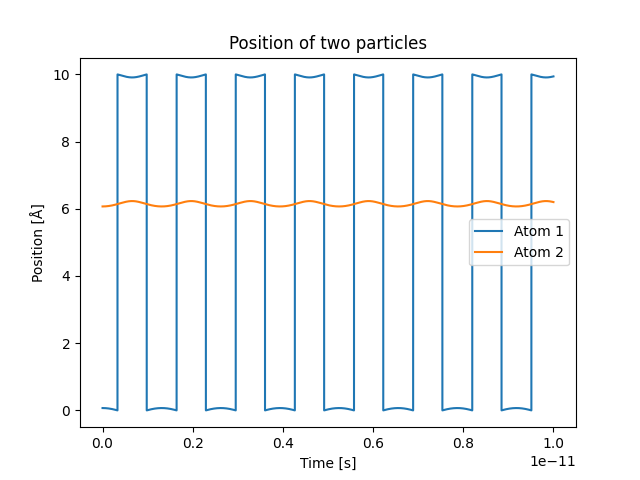
\includegraphics[width=\textwidth]{bsX.png}
        \caption{Position as a function of time $x(t)$ for the two atoms.}
        \label{fig: Position BT}
    \end{subfigure}
    \hfill
    \begin{subfigure}[b]{0.45\textwidth}
        \centering
        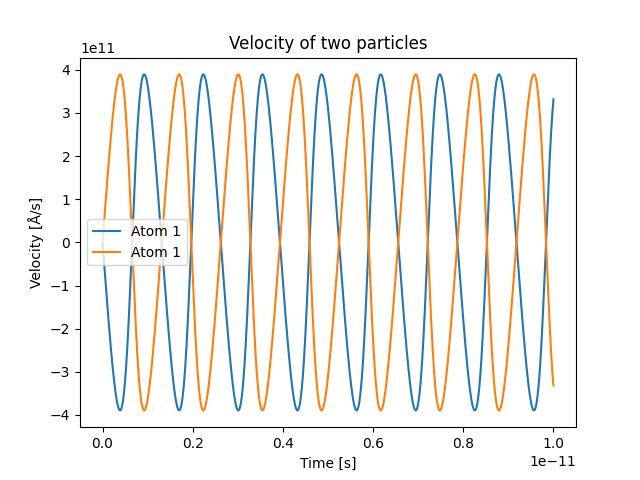
\includegraphics[width=\textwidth]{bsV.png}
        \caption{Velocity as a function of time $v_x(t)$ for the two atoms.}
        \label{fig: Velocity BT}
    \end{subfigure}
    \caption{(a) The atoms position and (b) velocity as a function of time.}
    \label{fig: Position & Velocity Bouncing test}
\end{figure}\noindent
The energy of the system is conserved, as seen by the constant Hamiltonian $\mathcal{H}(t)$ in figure \ref{fig: Energy Bouncing test}.
In the figure it's also shown that the kinetic energy, $\mathcal{K}(t)$ and the potential energy $\mathcal{V}(t)$ oscillates in time.
\begin{figure}[H]
    \centering
    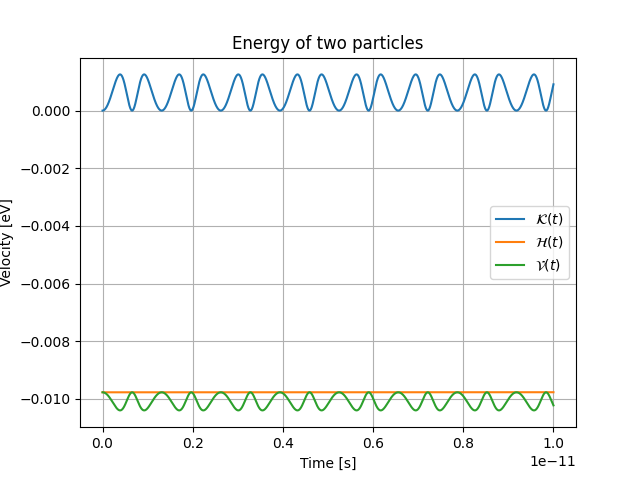
\includegraphics[scale = 0.5]{bsE.png}
    \caption{The energy in the system as a function of time.}
    \label{fig: Energy Bouncing test}
\end{figure}

\subsection{Gas}
The position of the atoms in the gas are distributed in a uniform manner, as seen in figure \ref{fig: initial position gas}. Here one has $n = 5$ atoms in each dimension, which results in total of $N = 125$ atoms. 
The box-length is determined to be $L = 18.09$~Å, and the density is set to be $\rho = 1.4$~g$/$l.
The atoms are given an initial velocity which is randomized, and the temperature is set to $94.4K$, via the velocity scaling discussed prior, eq \eqref{eq: velocity rescaling}.

\begin{figure}[H]
    \centering
    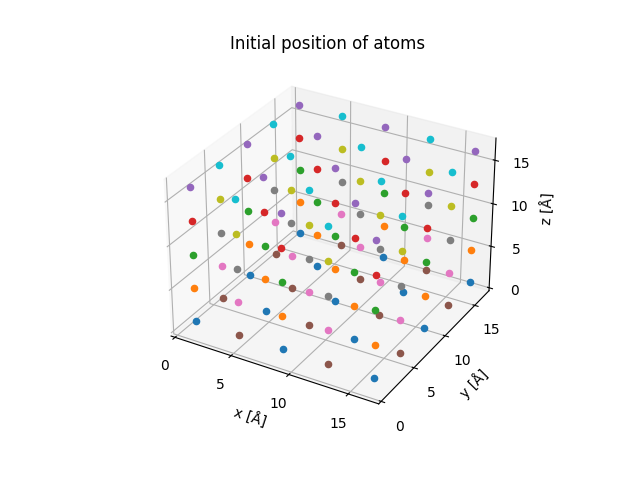
\includegraphics[scale = 0.5]{initial_position.png}
    \caption{The initial position of the atoms in the gas.}
    \label{fig: initial position gas}
\end{figure}\noindent
As seen in the above figure, one has not placed the atoms in a grid spanning the entire volume, but rather in a slightly bulked manner. This is to ensure that the position on the boundaries are not too close to the atoms in the next image, which would result in a stronger interaction between the atoms in the neighboring images.
This would result in a massive force between the atoms, thus also massive accelerations, which now is avoided.
The atoms in the layer closest to the boundary will have a strong interaction with the nearest image, and thus will show an oscillatory behavior in the position. A single atom in located in bottom $x-y$ plane oscillates in the $z$-direction, as seen in figure \ref{fig: z-direction-gas}.

\begin{figure}[H]
    \centering
    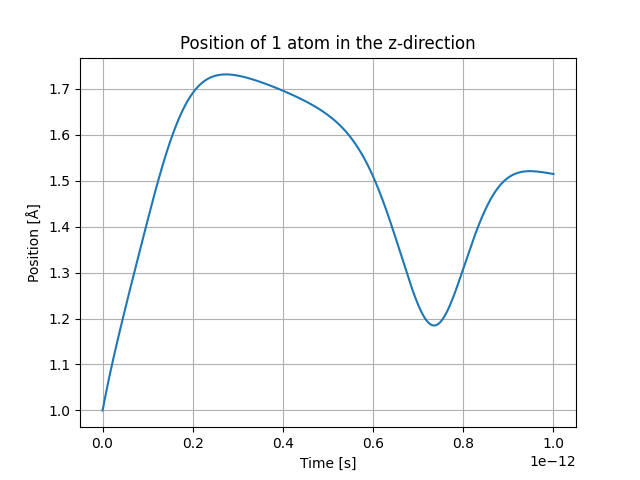
\includegraphics[scale = .5]{pos-z_direction.png}
    \caption{The position of the atom in the $z$-direction as a function of time.}
    \label{fig: z-direction-gas}
\end{figure}


\section{Conclusion}

\end{document}
 
